\documentclass[slidestop,usenames,dvipsnames]{beamer}
\usepackage[utf8]{inputenc}
\usepackage{fancyvrb}
\usepackage[absolute,overlay]{textpos}

\title{Commit Rater}
\subtitle{Analysis \& Synthesis}
\author{Marco Brack \and Carsten Hartenfels}
\date{2015-06-18}


\beamertemplatenavigationsymbolsempty
\usetheme{Boadilla}
\usecolortheme{whale}
\setbeamertemplate{itemize items}[default]
\setbeamertemplate{enumerate items}[default]
\defbeamertemplate*{footline}{my infolines theme} {
    \leavevmode
    \hbox{
    \begin{beamercolorbox}[wd=.333333\paperwidth,ht=2.25ex,dp=1ex,center]{author in head/foot}
        \usebeamerfont{author in head/foot}\insertshortauthor
    \end{beamercolorbox}
    \begin{beamercolorbox}[wd=.333333\paperwidth,ht=2.25ex,dp=1ex,center]{title in head/foot}
        \usebeamerfont{title in head/foot}\insertshorttitle
    \end{beamercolorbox}
    \begin{beamercolorbox}[wd=.309\paperwidth,ht=2.25ex,dp=1ex,center]{date in head/foot}
        \usebeamerfont{date in head/foot}\insertshortdate{}\hspace*{2em}
        \insertframenumber{} / \inserttotalframenumber\hspace*{2ex}
    \end{beamercolorbox}}
    \vskip0pt
}

\newcounter{FrameCounter}
\newcommand{\nextframe}[0]{\stepcounter{FrameCounter}}
\newcommand{\framecount}[1]{\frametitle{\arabic{FrameCounter}. {#1}}}
\newcommand{\fitem}{\pause\vfill\item}
\newcommand{\gitem}{\vfill\item}
\newcommand{\fimage}[2]{\pause\vfill\begin{center}\includegraphics[width={#2}]{#1}\end{center}}

\begin{document}

\begin{frame}
    \titlepage
    \begin{center}
        \url{https://github.com/hartenfels/Commit-Rater}
    \end{center}
\end{frame}


%%%%%%%%%%%%%%%%%%%%%%%%%%%%%%%%%%%%%%%%%%%%%%%%%


\begin{frame}
    \frametitle{Content}
    \begin{itemize}
        \gitem Previous Showcase
        \gitem New Research Goals
        \gitem Analysis
        \gitem Additional Analysis
        \gitem Synthesis
    \end{itemize}
\end{frame}


\nextframe
\begin{frame}
    \framecount{Previous Showcase}
    \vfill
    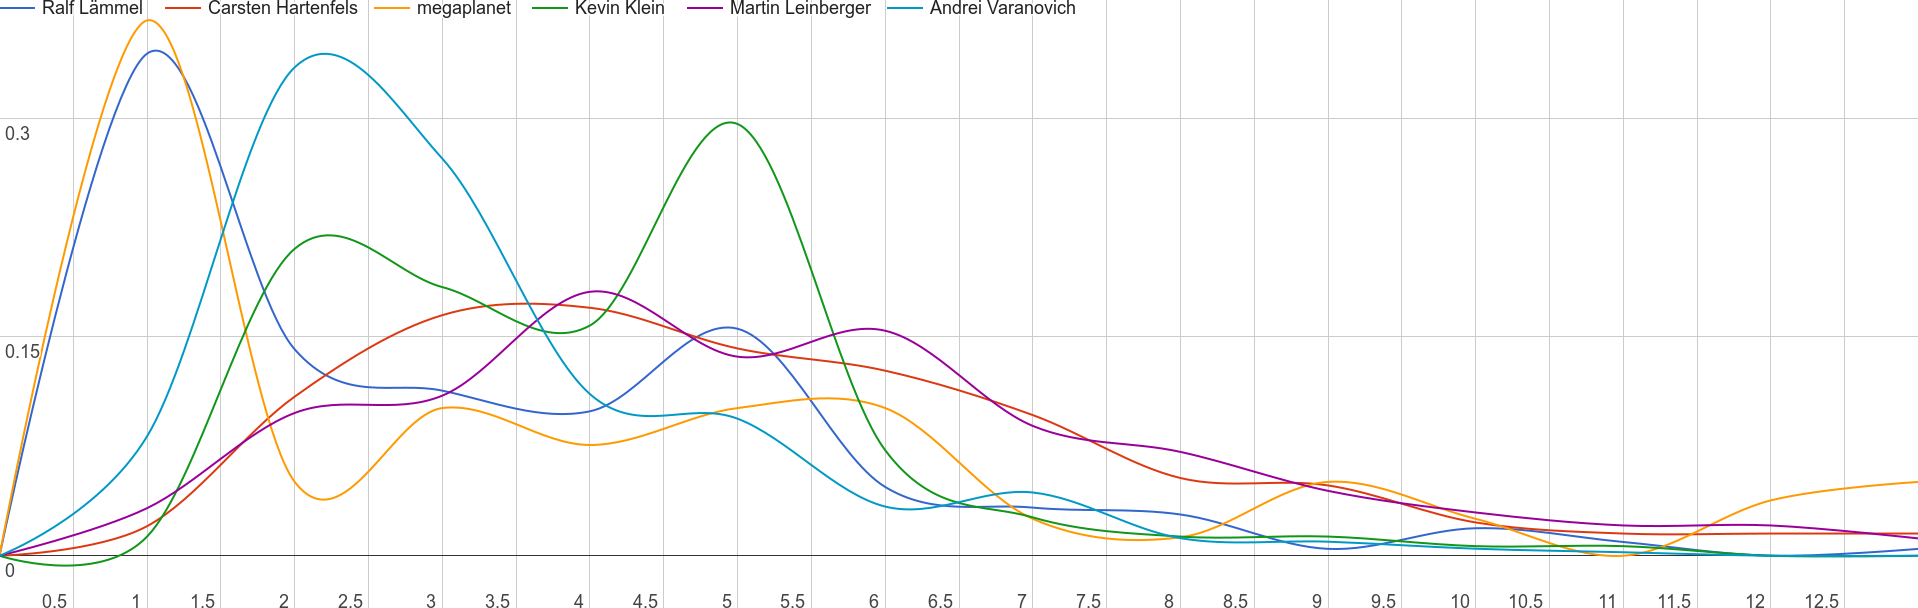
\includegraphics[width=\textwidth, clip=true, trim=0 0 700px 0]{img/101worker-wordCounts}
    \vfill
\end{frame}


\nextframe
\begin{frame}
    \framecount{New Research Goals}
    \begin{itemize}
        \fitem Recognize Good Commits
        \fitem Thereby Recognize ``Good Developers''
        \fitem Provide Feedback for Developer
        \fitem Rank Developers for the Lulz
    \end{itemize}
\end{frame}


\nextframe
\begin{frame}
  % Taken from http://chris.beams.io/posts/git-commit/#seven-rules
    \framecount{Analysis}
    \begin{itemize}
        \fitem Separate subject from body with a blank line
        \fitem Limit the subject line to 50 characters
        \fitem Capitalize the subject line
        \fitem Do not end the subject line with a period
        \fitem Use the imperative mood in the subject line
        \fitem Wrap the body at 72 characters
        \fitem Use the body to explain what and why vs. how
    \end{itemize}
\end{frame}


\nextframe
\begin{frame}
    \framecount{Additional Analysis}
    Not factored into rating
    \begin{itemize}
        \fitem Trailing Whitespaces
        \fitem Spelling
        \fitem Vulgarity
        \fitem Word Count
        \fitem Whitespace Changes
        \fitem Lines/Files Changed
    \end{itemize}
\end{frame}


\nextframe
\begin{frame}
    \framecount{Synthesis}
    \begin{itemize}
        \fitem Take Binary Analysis Results for Each Commit
        \fitem Apply Arbitrary (or Customizable) Weights
        \fitem Add Together, Maybe Normalize
        \fitem Calculate Average
    \end{itemize}
\end{frame}


%\nextframe
%\begin{frame}
%    \framecount{Possible Evaluation}
%    \begin{itemize}
%        \fitem Guess a Ranking Threshold
%        \fitem Assign \emph{Good} or \emph{Bad} Based on that Threshold
%        \fitem Let Real People Assign \emph{Good} or \emph{Bad} to Developers
%        \fitem Compare Results (By Statistical Analysis)
%    \end{itemize}
%\end{frame}


%%%%%%%%%%%%%%%%%%%%%%%%%%%%%%%%%%%%%%%%%%%%%%%%%


\nextframe
\begin{frame}
    \vfill
    \begin{center}
        $~$\\
        $~$\\
        {\Huge Thank You All For Listening}\\
        $~$\\
        $~$\\
        \url{https://github.com/hartenfels/Commit-Rater}
    \end{center}
\end{frame}

\end{document}
